\chapter{System Design}
\label{ch:SystemDesign}

After analyzing functional and nonfunctional requirements, identifying use cases and possible usage scenarios, this chapter focusses on creating a system design model derived from the specifications of the analysis model. The resulting system design artifact forms the foundation for the subsequent object design analysis.

In order to achieve the best possible quality of our proposed system and its output, the criteria identified from Section \ref{sec:Requirements} must be evaluated and balanced with regard to their applicability. Demands that have not been considered up to now as well as contradicting requirements must be incorporated or resolved. Therefore, the design goals of our system are defined in Section \ref{sec:DesignGoals} and prioritized to maximizie the possible benefit for all stakeholders. 

Considering all functionality and quality criteria defined during requirements analysis results in a complex system that is difficult to develop and maintain as a whole. In order to distribute the workload among development teams and to facilitate training of new team members, subsystems need to be identified that support a clear separation of concerns and can be maintained independently. We identified a composition of subsystems in which each subsystem provides well-defined interfaces to its encapsulated internal functionality. Section \ref{sec:SubsystemDecomposition} contains the details of the interactions between subsystems and gives an overview of the modular architecture of our proposed system.

Our system is supposed to be executed as an additional step during the build stage in an existing CI/CD pipeline. While it is designed to run automatically, various boundary conditions require manual intervention of the user in order to resolve errors in the configuration or during runtime. Integrating the system into an existing CI/CD pipeline and troubleshooting for occuring errors is described in detail in Section \ref{sec:BoundaryConditions}.

In Section \ref{sec:HardwareSoftwareMapping} an exemplatory execution environment is used to demonstrate the flexibility of the subsystem decomposition. Therefore, its abstract components are mapped to representational subsystems that could be applied in this execution environment. In addition, all modified services and resulting artifacts are described in detail.
\newpage
\section{Design Goals}
\label{sec:DesignGoals}

The main purpose of our system is to facilitate the evolution process of Web APIs. Therefore, it must meet several requirements in order to be of real benefit to all actors involved. Some of these requirements are not complementary but contradict each other. In order to achieve the best possible result for our users, we prioritize our design decisions in the following section.

\paragraph{Dependability Criteria}
Decisions about the dependability of the system concern the effort to be invested in minimizing system crashes and their effects on users \cite{bruegge_object-oriented_2010}. Integrating our system into the CI/CD pipeline of an application means that subsequent process steps rely on its error-free execution. Emphasis is therefore on \ref{nfr:TestCoverage} which implies creating extensive tests of the migration logic, especially with regard to edge cases. In addition, incorrect user input must be handled and detailed error messages must be provided so that users can identify and correct errors themselves. By prioritizing robustness and fault tolerance, the delivery time for new functionality in our system, such as additional language or API type support, is significantly extended. 

Furthermore, client applications rely on an error-free execution of the code emitted by our system. Therefore, the resulting library code needs to handle internal errors appropriately and forward any response emitted by the Web API.  As it is designed to mirror the behavior of the Web API, also any errors that are issued by the Web API are returned to the requesting method within client code. Hence, client developers are responsible for handling errors appropriately and designing their application for failures. 

\paragraph{Performance Criteria}
Achieving high performance measures is not an essential requirement of our system as it runs as a background process in an application's CI/CD pipeline or in a user's local terminal. While users do not depend on fast response times or a high throughput, the memory usage of our system increases with the size of the IDL document or migration manual. Therefore, when designing the system architecture, care should be taken that memory-intensive components are encapsulated as this provides the possibility to replace them with more efficient algorithms if necessary. In terms of the library code generated, our design choices \ref{fr:Facade} and \ref{fr:AdaptFacade} result in decreased performance for client applications as API requests and responses must be processed across multiple layers.

\paragraph{Maintenance Criteria}
According to Bruegge et. al, maintenance design decisions determine the difficulty of changing a system after its initial deployment \cite{bruegge_object-oriented_2010}. Well-defined subsystems that enable a clear separation of concerns ensure that our system maintains a high degree of extensibility and modifiability. In particular, components concerned with the language-specific generation of libraries or the import of different types of IDLs must be designed with strict consideration of extensibility. This is due to the fact that supporting more languages and types of APIs is critical to increasing our system's adoption and adding additional value to its users. The encapsulation of language or API-specific functionality also improves the modifiability of our system by limiting changes due to external influences to the corresponding component. 

Focussing on expandability and modifiability involves a trade-off in terms of portability and adaptability. Adapting the system to another application domain, e.g. managing API evolution for providers is not intended. Furthermore, the support of different types of language-specific library generation for several Web API styles increases the complexity of the system, which means that the effort for new maintainers to understand the system is increased. Porting it to other platforms which implies using a different host language becomes more complicated. 

Although we do not consider any cost criteria in this thesis, it is important to note that our maintenance criteria together with an extensive testing result in longer delivery times with significantly higher costs for development and maintenance. Using the output of our system, on the other hand, reduces development costs and delivery times of client applications, as switching between different API types and programming languages is frictionless, an according implementation of our system implied. In order to be able to use the generated code for a different application domain, programming language or API type, our system just requires the corresponding parameters and does not need any adaptation of its functionality.

\paragraph{End User Criteria}
Reducing the manual overhead of evolution for Web API consumers is the main goal of our proposed system. Automating the workflow for migrating client applications adds an additional task for Web API providers. By requiring them to specify all changes in a migration guide for each release, the effort of consumers is shifted to the provider side. This design decision was made based on the assumption that future research can concentrate on automating the creation of a migration guide for Web API providers. Related research as shown in section \ref{sec:APIEvolutionAutomation} demonstrates how capturing and replaying or comparing techniques can be used to realize possible scenarios like scenario \ref{subsubsec:Scenario:graphQLScenario}. In addition, the number of consumers of public Web APIs is exceeding their providers, resulting in an overall reduction in maintenance effort. 

To maximize the positive impact of the system, special attention is paid to its usability for Web API consumers. Nonfunctional requirements were specified for coloring of key output messages (\ref{nfr:Coloring}), documentation of generated library code (\ref{nfr:ClientDocumentation}) and provision of help messages (\ref{nfr:Help}) to ensure a high degree of usability. All of the code emitted by our system is documented by code comments that explain how to use the Web API thus facilitating learning for users.
\newpage
\section{Subsystem Decomposition}
\label{sec:SubsystemDecomposition}

By dividing our system into smaller subsystems, the workload can be distributed among development teams and components that are already available to developers can be reused. The subsystems were identified by analyzing the flow of events shown in Figure \ref{fig:useCaseConsumer} and \ref{fig:useCaseProvider}. Each subsystem has precisely defined interfaces that are provided to its consumers and thus enable a modular architecture in which subsystems can easily be replaced by more efficient alternatives. Furthermore, our design enables implementations that support importing multiple IDL types and generating output for multiple programming languages at the same time. 

\begin{figure}[h]
	\centering{
		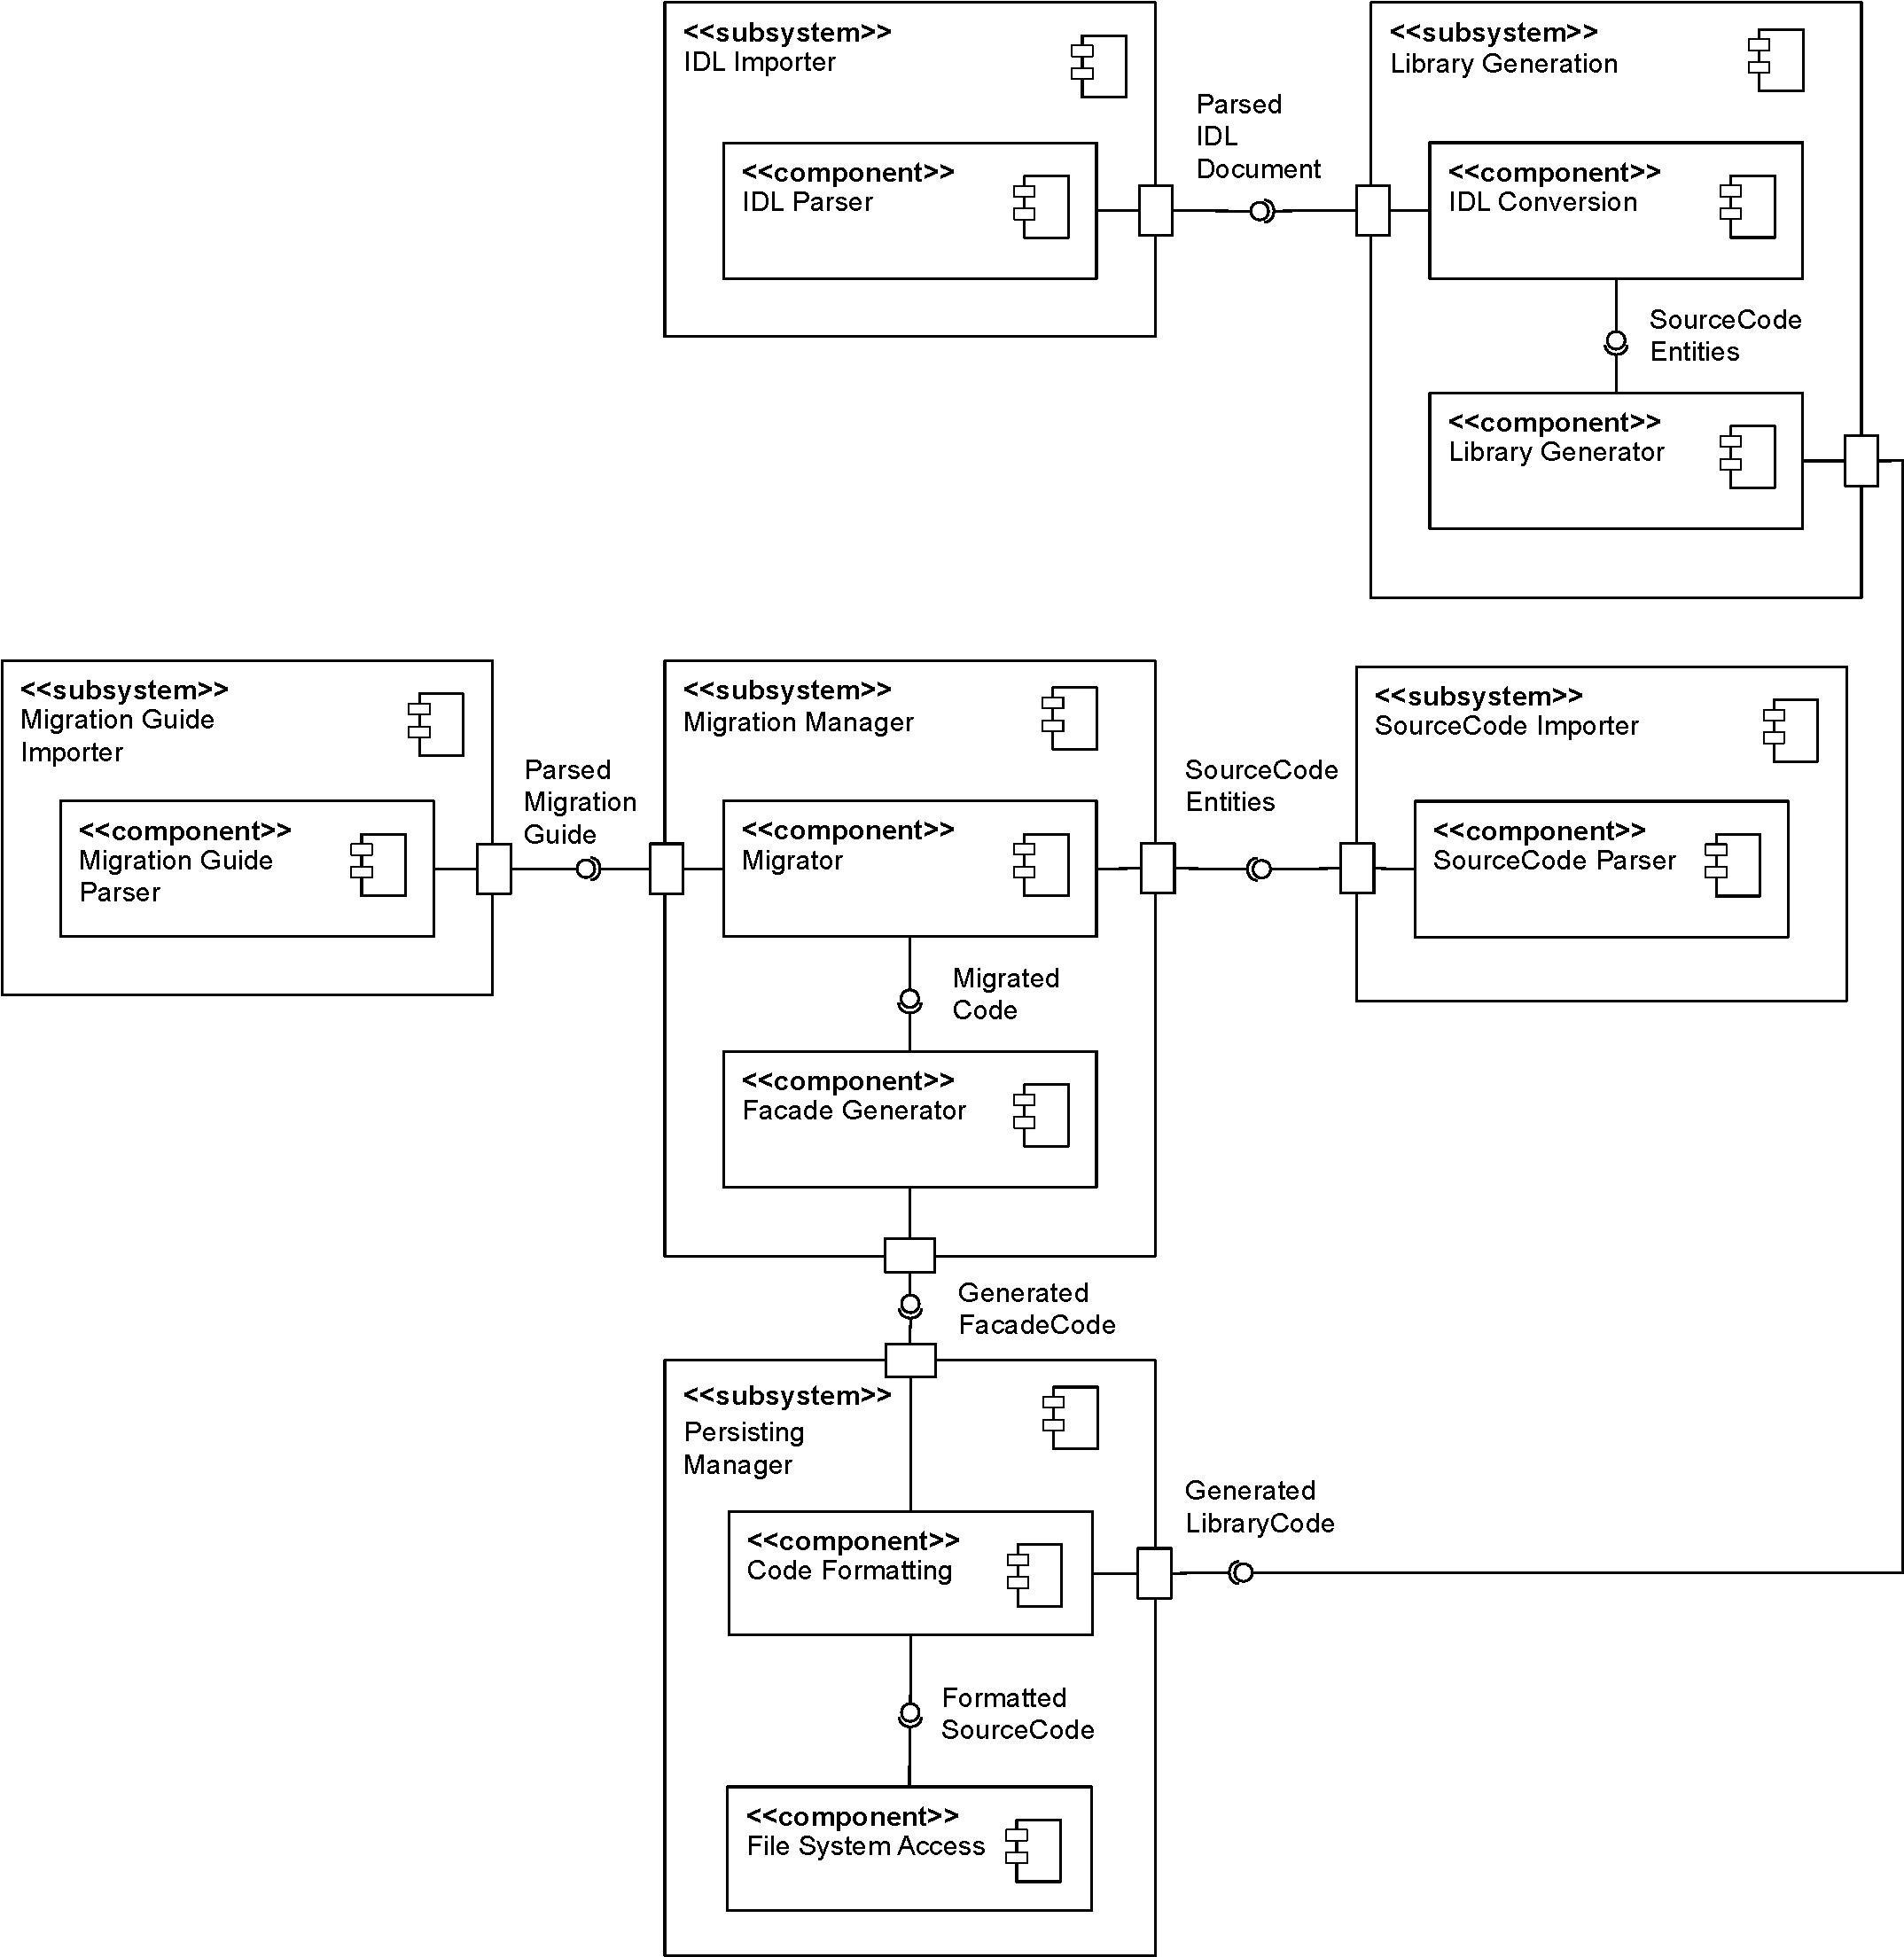
\includegraphics[width=155mm]{images/subsystem_decomposition.pdf}
		\caption{Subsystem decomposition}
		\label{fig:subsystemDecomposition}
	}
\end{figure}

For creating the library and persistent facade subsystem as shown in Figure \ref{fig:outcome}, various tasks need to be executed in order to generate them from IDL documents, previous versions of them and a machine-readable migration guide. 

In order to generate the library subsystem an IDL document must be imported and converted into the source code of a specific programming language. Therefore, a dedicated \texttt{IDL} \texttt{Importer} subsystem for reading and parsing of an IDL document supplies its encoded representation to the \texttt{Library} \texttt{Generation} subsystem. This converts the encoded IDL document into a textual representation of source code of a selected programming language. 

Creating the persistent facade subsystem requires the interaction of several resources that have to be imported first. Our migration guide as shown in Figure \ref{fig:migGuide} includes any changes made to the Web API between the previous and current versions. The corresponding \texttt{Migration} \texttt{Guide} \texttt{Importer} subsystem handles all of the tasks related to fetching, parsing, and validating a migration guide. It provides the parsed representation of the document to the \texttt{Migration} subsystem. For some types of changes, missing information is too cumbersome to be defined in a migration guide and cannot be implicitly derived from an IDL document. Therefore, the source code of the previous version of the facade subsystem must be analyzed to obtain this information. The \texttt{SourceCode} \texttt{Importer} subsystem reads and parses all files of the previous facade and library to provide the encoded result to the \texttt{Migration} subsystem. The \texttt{Migrator} component uses the received information to adapt the previous version of the facade using the changes as stated in the migration guide. Its output is used by the \texttt{Facade} \texttt{Generator} component to generate a textual representation of source code in the desired programming language. 

The emitted source code from both subsystems, \texttt{Migration} and \texttt{Library} \texttt{Gen\-er\-a\-tion}, is used by the \texttt{Persisting} \texttt{Manager} subsystem which formats the code according to a user-defined linting rule set. The formatted source code is written to file using the \texttt{File} \texttt{System} \texttt{Access} component.



\section{Boundary Conditions}
\label{sec:BoundaryConditions}

When using our proposed system, various boundary conditions regarding integration and execution must be taken into account. It is designed to be integrated into an existing CI/CD pipeline of a client application but can also be run locally via a CLI. When it is used as a step in an existing CI/CD pipeline, it must be part of a stage prior to releasing in order to ensure that the most recent version of the Web API is used. Client developers must specify multiple configuration parameters to setup the system. While configuring a migration strategy and specifying a target programming language are mandatory tasks, users can optionally define a linting rule set which determines the code formatting of the emitted code. 

On its initial run, our proposed system does not require a migration guide as the latest version of the Web API is used as a starting point for generating the persistent facade. Hence, only the \ac{URI} of the IDL document needs to be present. After that, each run requires specifying the \acp{URI} of both, the IDL document and the migration guide in order to adapt the facade and update the library subsystems. Omitting mandatory parameters results in an error message during runtime that highlights the missing configuration. Optional parameters do not trigger error messages as a default configuration is used instead. Detecting missing configuration parameters and specifying error messages are tasks of the \texttt{Executable} subsystem.

In addition to configuration parameters, unmet preconditions also raise errors. If the system fails to fetch either the IDL document or the migration guide, no output can be generated and execution will be aborted. The specific reason for the failure is given in the CI/CD system's log or on the command line. Furthermore, if changes specified in the migration guide are incompatible or inconsistent, the facade adaptation will fail and an error message will be logged. Removing a parameter from a non-parameterized method or adding and removing the same parameter to and from a method at the same time are examples of incompatible or inconsistent changes, respectively. Errors related to fetching and parsing of an IDL document or migration guide are managed by the \texttt{IDL} \texttt{Importer} subsystem and \texttt{Migration} \texttt{Guide} \texttt{Importer} subsystem. Checking for incompatibilities and inconsistencies within the migration guide is done by the \texttt{Migrator} component.




\section{Hardware-Software Mapping}
\label{sec:HardwareSoftwareMapping}

For better understanding, in this section the abstract components as shown in Figure \ref{fig:subsystemDecomposition} are mapped to concrete components in an exemplatory execution environment. Therefore, the target client environment is defined as the Apple ecosystem, particularly the development of iOS, iPadOS or macOS-based client applications.  A common use case for this environment is the integration of resource-based Web APIs in the REST architectural style that are described by the OpenAPI \ac{IDL}. Swift is used as the target programming language in which to output the result and to import previous versions of the facade code. By restricting to these criteria, the subsystem decomposition now contains more specific components as shown in Figure \ref{fig:subsystemConcrete}. 

\begin{figure}[!h]
	\centering{
		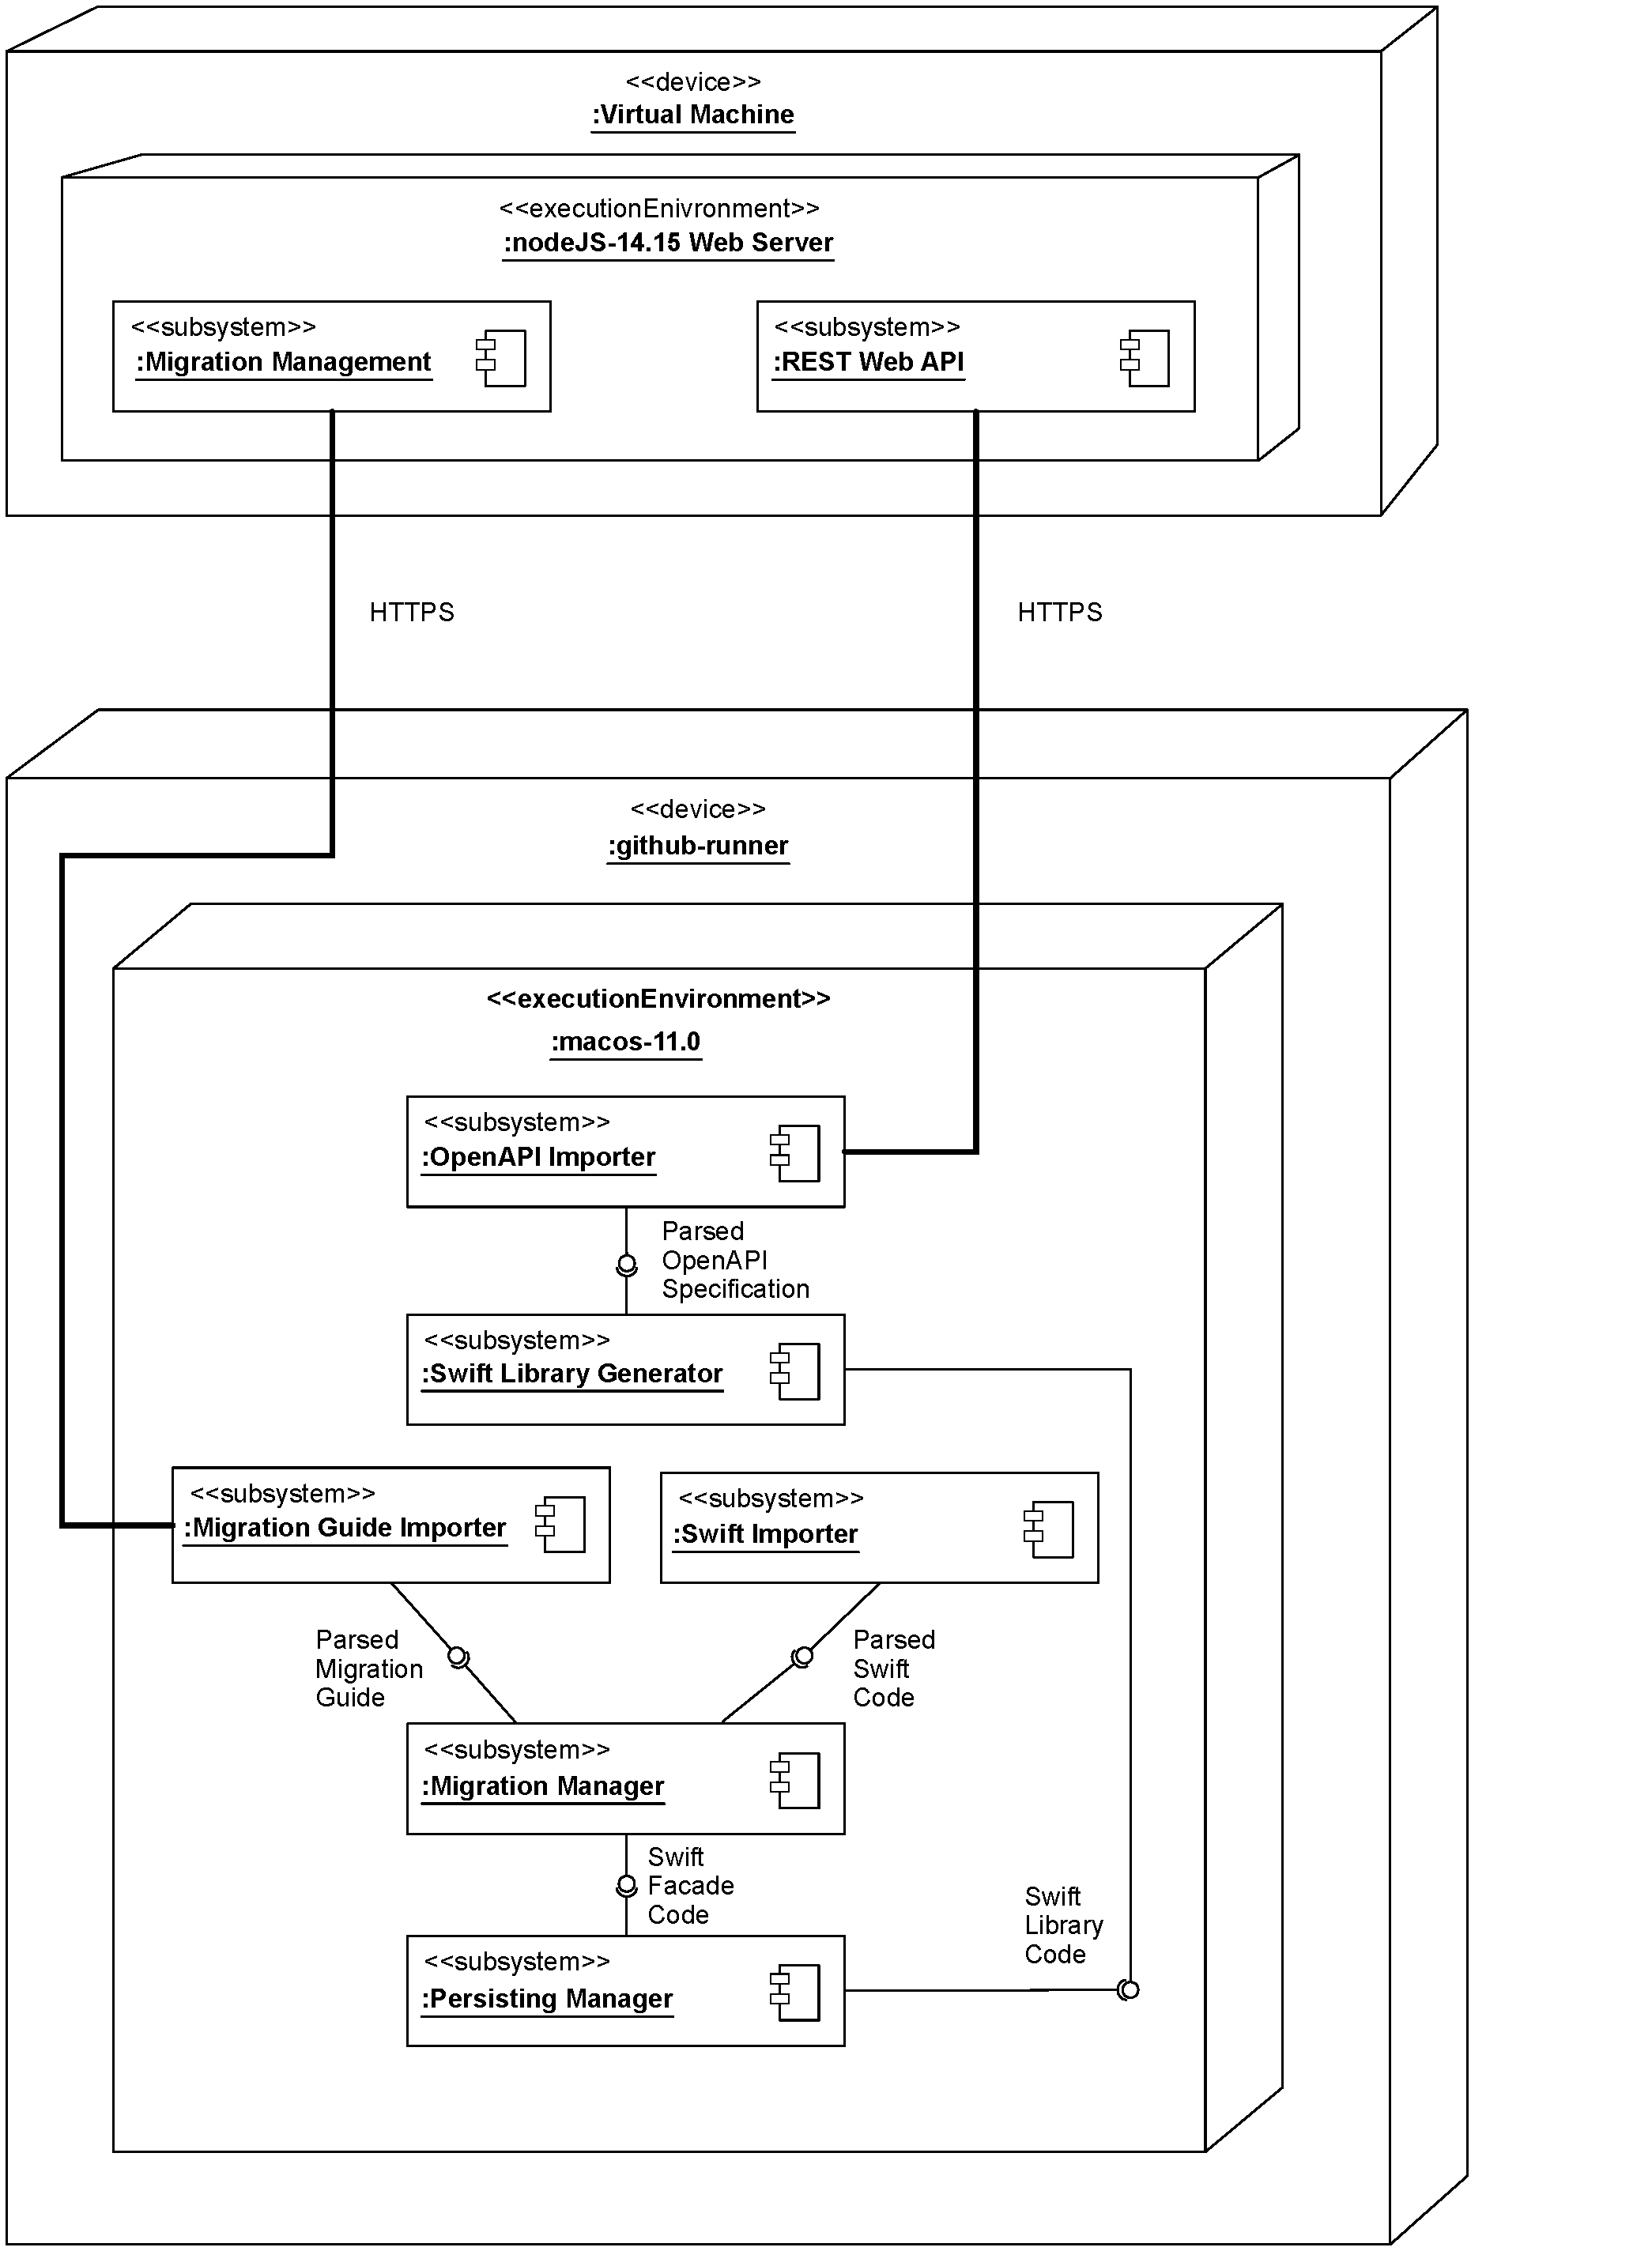
\includegraphics[width=150mm]{images/subsystem_concrete.pdf}
		\caption{Subsystem decomposition in an Apple ecosystem}
		\label{fig:subsystemConcrete}
	}
\end{figure}

The Web API is built using the \ac{REST} architectural style. It is served by a \texttt{nodeJS} web server hosted on a virtual machine maintained by the Web API provider. Its functionality is described using the OpenAPI \ac{IDL}. This document is published on a separate URI of the Web API. Additionally, a \texttt{Migration Management} subsystem is used to track all changes that have been introduced to the Web API. It notes all changes in a machine-readable migration guide and publishes it on a separate URI. Both document can be retrieved using \texttt{HTTPS}. 

To import the specification document, the OpenAPI Importer subsystem must be able to parse specifications using both, the \textit{\ac{JSON}} and \textit{\ac{YAML}} documentation styles. While the system itself can be implemented using an arbitrary programming language, every subsystem that is concerned with importing or generating source code must support Swift. The \texttt{Swift} \texttt{Library} \texttt{Gen\-er\-ation} subsystem uses the parsed specification to create Swift files containing model and endpoint definitions that enable the interaction with the Web API. Appropriate tooling to generate a library from an OpenAPI specification is available for all major programming languages. The OpenAPI Generator\footnote{https://openapi-generator.tech/}, implemented using Java, is one of them, supporting 65 programming languages and dialects. It combines the functionality of the \texttt{OpenAPI} \texttt{Importer} and \texttt{Swift} \texttt{Library} \texttt{Gen\-er\-ation} subsystems.

Parsing a migration guide requires a custom implementation of the \texttt{Migration} \texttt{Guide} \texttt{Importer} as no reusable components exist yet. The subsystem responsible for importing the previous facade must support parsing Swift code. The internal behavior of it is modified according to the changes as stated in the encoded migration guide. After that, the adapted facade is transformed into the textual representation of Swift-based source code by the \texttt{Swift} \texttt{Facade} \texttt{Generator}. There are multiple tools available that support generating Swift code using Stencil templates. The most popular ones are SwiftGen\footnote{https://github.com/SwiftGen/SwiftGen} and Sourcery\footnote{https://github.com/krzysztofzablocki/Sourcery}. They provide similar features that enable users to generate Swift code based on several template types by executing the compiled application via CLI. Sourcery additionally offers a well-maintained framework to enable an integration into existing Swift applications.

The \texttt{Persisting} \texttt{Manager} subsystem uses a linting ruleset to format the library and facade code according to its configuration, before adding meta-files and creating a Swift package which can be imported by client applications using the \textit{\ac{SPM}}. Formatting code based on a linting ruleset is one feature of SwiftLint\footnote{https://github.com/realm/SwiftLint}, the most popular linter for Swift code. While it can be installed and used via CLI, it also supports an integration as a Swift package that enables developers to lint and format Swift code stored in its textual representation.
